\documentclass[tikz,border=2pt]{standalone}
\usepackage{amsmath,amssymb}
\usepackage{tikz}
\usetikzlibrary{arrows.meta}

\begin{document}
% A diagonal matrix scales each coordinate axis separately: the unit square becomes an
% axis-parallel rectangle.
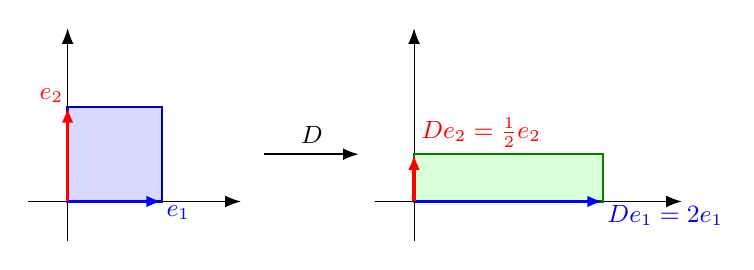
\begin{tikzpicture}[every node/.style={font=\small}, >={Latex[length=2mm]}]
	\draw[->] (-0.5,0) -- (2.2,0);
	\draw[->] (0,-0.5) -- (0,2.2);
	\fill[blue!15] (0,0) rectangle (1.2,1.2);
	\draw[blue!70!black, thick] (0,0) rectangle (1.2,1.2);
	\draw[->, blue, very thick] (0,0) -- (1.2,0) node[below right, inner sep=1pt] {$e_1$};
	\draw[->, red, very thick] (0,0) -- (0,1.2) node[above left, inner sep=1pt] {$e_2$};
	\draw[->, thick] (2.5,0.6) -- (3.7,0.6) node[midway, above] {$D$};
	\begin{scope}[xshift=4.4cm]
		\draw[->] (-0.5,0) -- (3.4,0);
		\draw[->] (0,-0.5) -- (0,2.2);
		\fill[green!15] (0,0) rectangle (2.4,0.6);
		\draw[green!50!black, thick] (0,0) rectangle (2.4,0.6);
		\draw[->, blue, very thick] (0,0) -- (2.4,0) node[below right, inner sep=1pt] {$De_1=2e_1$};
		\draw[->, red, very thick] (0,0) -- (0,0.6) node[above right, inner sep=2pt] {$De_2=\tfrac12e_2$};
	\end{scope}
\end{tikzpicture}
\end{document}
